\documentclass[tikz,border=0pt]{standalone}
\pdfminorversion=7
\usepackage[T1]{fontenc}
\usepackage{lmodern,amsmath,amssymb,graphicx}
\usepackage{pgfplots}
\usetikzlibrary{arrows.meta,calc,positioning,patterns,decorations.pathreplacing}
\pgfplotsset{compat=1.18}
\definecolor{family}{RGB}{0,140,18}
\definecolor{familypale}{RGB}{225,255,226}
\definecolor{frozen}{RGB}{49,57,208}
\definecolor{frozenpale}{RGB}{234,235,255}
\definecolor{adapter}{RGB}{219,102,0}
\definecolor{adapterpale}{RGB}{255,196,135}
\definecolor{outputcol}{RGB}{120,38,130}
\definecolor{ink}{RGB}{33,33,33}
\definecolor{muted}{RGB}{105,105,105}
\tikzset{
 figure/.style={x=1pt,y=1pt,line cap=round,line join=round,text=ink,
   >={Stealth[length=7pt,width=6pt]},font=\fontsize{20}{24}\selectfont},
 title/.style={font=\fontsize{29}{33}\selectfont},
 heading/.style={font=\fontsize{22}{26}\selectfont},
 labeltext/.style={font=\fontsize{18}{22}\selectfont,align=center},
 smalllabel/.style={font=\fontsize{15}{19}\selectfont,align=center},
 equation/.style={font=\fontsize{24}{29}\selectfont,align=center},
 flow/.style={->,line width=1.3pt},
 fineflow/.style={->,line width=.8pt},
 target/.style={circle,fill=family,draw=white,line width=1.2pt,inner sep=0pt,minimum size=12pt},
 candidate/.style={circle,fill=white,draw=muted,line width=1.3pt,inner sep=0pt,minimum size=10pt},
 neuron/.style={circle,draw=frozen,fill=frozen!18,minimum size=13pt,inner sep=0pt,line width=.8pt}
}
\DeclareMathOperator{\rank}{rank}
\DeclareMathOperator{\row}{row}
\DeclareMathOperator{\col}{col}
\newcommand{\R}{\mathbb R}
\graphicspath{{assets/}}
\newcommand{\canvas}[1]{\path[use as bounding box] (0,0) rectangle (960,600);
  \node[title,anchor=west] at (36,557) {#1};}
\newcommand{\glyphgrid}[2]{
 \begin{scope}[shift={(#1,#2)}]
  \fill[white] (0,0) rectangle (136,136);
  \foreach \x/\y/\c in {1/1/80,2/2/80,2/3/45,3/4/45,3/5/45,4/5/100,4/6/45,5/6/45,5/4/45,5/2/100,6/1/80}{
    \fill[frozen!\c] (\x*17,\y*17) rectangle ++(17,17);
  }
  \draw[step=17pt,black!30,line width=.35pt] (0,0) grid (136,136);
  \draw[black!45,line width=.6pt] (0,0) rectangle (136,136);
 \end{scope}}

\begin{document}
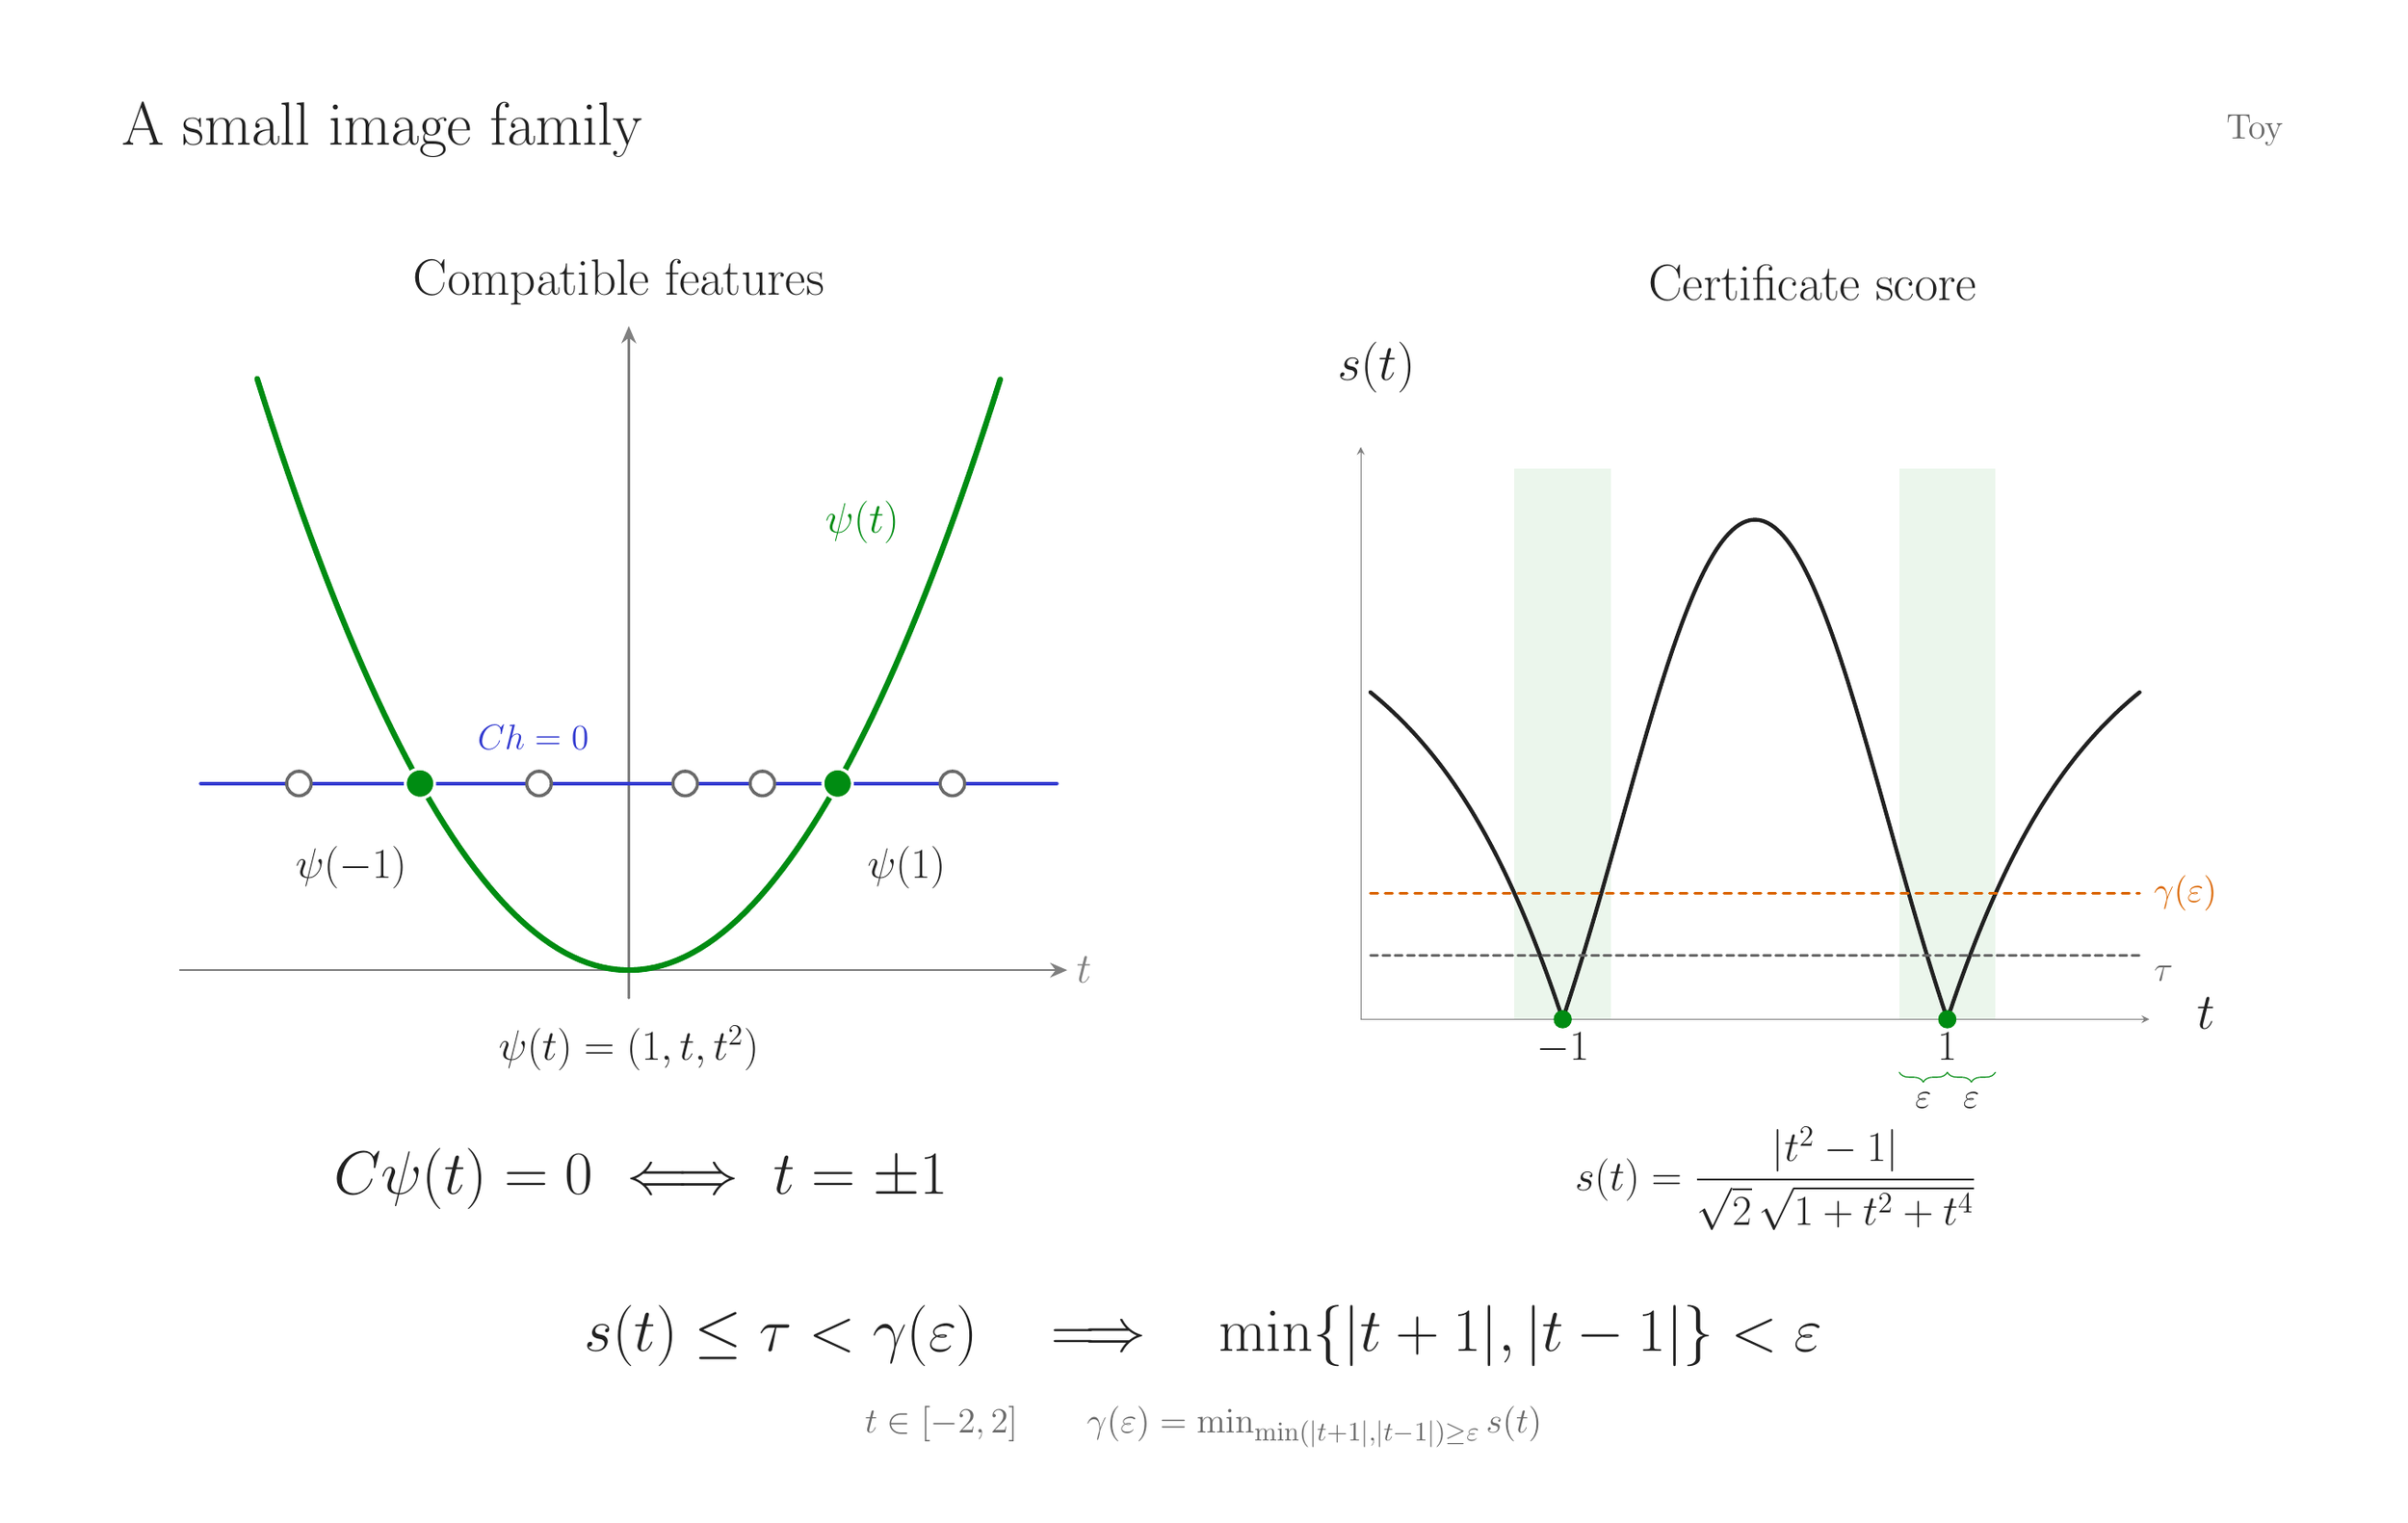
\begin{tikzpicture}[figure]
\canvas{A small image family}
\node[smalllabel,text=muted,anchor=east] at (923,557) {Toy};
\node[heading] at (242,495) {Compatible features};
\node[heading] at (728,495) {Certificate score};
\begin{scope}[shift={(246,215)},x=85pt,y=76pt]
 \draw[fineflow,black!50] (-2.15,0)--(2.1,0) node[right,labeltext] {$t$};
 \draw[fineflow,black!50] (0,-.15)--(0,3.45);
 \draw[line width=1.5pt,frozen] (-2.05,1)--(2.05,1);
 \node[smalllabel,text=frozen,anchor=east] at (-.15,1.25) {$Ch=0$};
 \draw[draw=family,line width=2.3pt,domain=-1.78:1.78,samples=100] plot (\x,{\x*\x});
 \node[labeltext,text=family,anchor=west] at (.9,2.4) {$\psi(t)$};
 \foreach \x in {-.43,.27,.64,-1.58,1.55} \node[candidate] at (\x,1) {};
 \node[target] at (-1,1) {};
 \node[target] at (1,1) {};
 \node[labeltext] at (-1.33,.55) {$\psi(-1)$};
 \node[labeltext] at (1.33,.55) {$\psi(1)$};
 \node[labeltext] at (0,-.42) {$\psi(t)=(1,t,t^2)$};
\end{scope}
\begin{axis}[
 at={(544pt,195pt)},anchor=south west,
 width=366pt,height=278pt,
 axis lines=left,axis line style={black!50,thin},
 xmin=-2.05,xmax=2.05,ymin=0,ymax=.81,
 xtick={-1,1},xticklabels={$-1$,$1$},ytick=\empty,
 tick label style={font=\fontsize{17}{20}\selectfont},
 xlabel={$t$},xlabel style={at={(axis description cs:1.05,0.01)},anchor=west},
 ylabel={$s(t)$},ylabel style={rotate=-90,at={(axis description cs:.02,1.08)},anchor=south},
 clip=false]
 \path[fill=family!8] (axis cs:-1.25,0) rectangle (axis cs:-.75,.78);
 \path[fill=family!8] (axis cs:.75,0) rectangle (axis cs:1.25,.78);
 \addplot[ink,line width=1.6pt,domain=-2:2,samples=241] {abs(x*x-1)/(sqrt(2)*sqrt(1+x*x+x*x*x*x))};
 \addplot[adapter,line width=1.1pt,dashed,domain=-2:2] {(1.25^2-1)/(sqrt(2)*sqrt(1+1.25^2+1.25^4))};
 \addplot[black!60,line width=1pt,densely dashed,domain=-2:2] {.09};
 \node[smalllabel,text=adapter,anchor=west] at (axis cs:2.03,.17781) {$\gamma(\varepsilon)$};
 \node[smalllabel,text=muted,anchor=west] at (axis cs:2.03,.065) {$\tau$};
 \addplot[only marks,mark=*,mark size=3.5pt,color=family] coordinates {(-1,0) (1,0)};
 \draw[decorate,decoration={brace,mirror,amplitude=4pt},draw=family] (axis cs:.75,-.075)--(axis cs:1,-.075)
  node[midway,below=5pt,smalllabel] {$\varepsilon$};
 \draw[decorate,decoration={brace,mirror,amplitude=4pt},draw=family] (axis cs:1,-.075)--(axis cs:1.25,-.075)
  node[midway,below=5pt,smalllabel] {$\varepsilon$};
\end{axis}
\node[equation] at (251,130) {$C\psi(t)=0\iff t=\pm1$};
\node[labeltext] at (713,130) {$s(t)=\dfrac{|t^2-1|}{\sqrt2\,\sqrt{1+t^2+t^4}}$};
\node[equation] at (480,66) {$s(t)\le\tau<\gamma(\varepsilon)\quad\Longrightarrow\quad
 \min\{|t+1|,|t-1|\}<\varepsilon$};
\node[smalllabel,text=muted] at (480,29) {$t\in[-2,2]\qquad\gamma(\varepsilon)=
 \min_{\min(|t+1|,|t-1|)\ge\varepsilon}s(t)$};
\end{tikzpicture}
\end{document}
